\section{Introduction}

%\subsection{Human-robot collaboration}

\begin{frame}{Human-robot collaboration}{Introduction}

\begin{columns}

\column{0.4\textwidth}
\begin{minipage}{\textwidth}
\begin{figure}
\centering
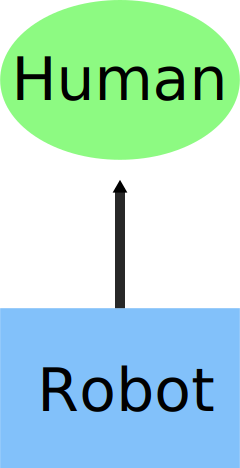
\includegraphics[width = 0.34\textwidth]{./figure/HR_org_chart1}
\end{figure}
\end{minipage}

\column{0.15\textwidth}
\begin{minipage}{\textwidth}
\begin{figure}
\centering
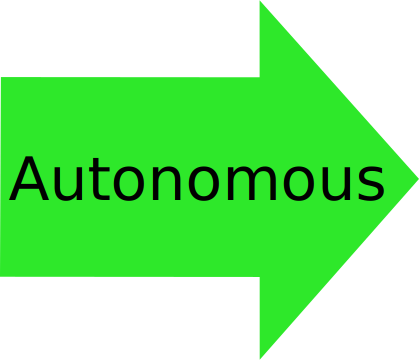
\includegraphics[width = 0.9\textwidth]{./figure/arrow_autonomous}
\end{figure}
\end{minipage}

\column{0.45\textwidth}
\begin{minipage}{\textwidth}
\begin{figure}
\centering
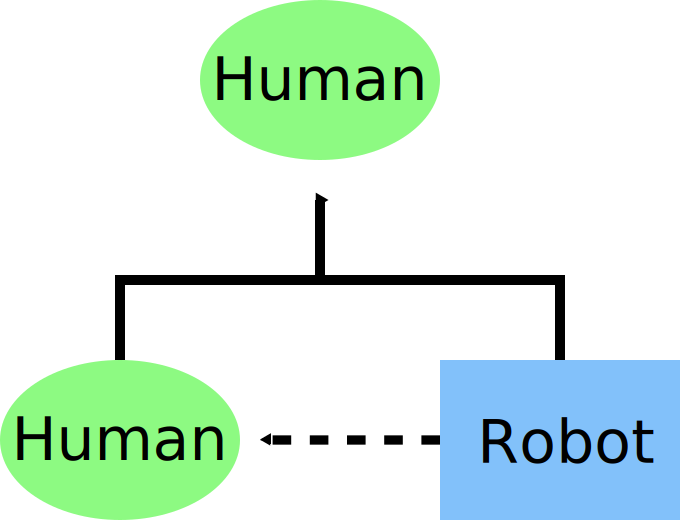
\includegraphics[width = 0.8\textwidth]{./figure/HR_org_chart2}
\end{figure}
\end{minipage}

\end{columns}

\bigskip

\begin{columns}

\column{0.4\textwidth}
\begin{center}
\textbf{Human-robot interaction}
\end{center}

\column{0.15\textwidth}

\column{0.45\textwidth}
\begin{center}
\textbf{Human-robot collaboration}
\end{center}

\end{columns}

\end{frame}

%\subsection{Cordon and search}

\begin{frame}{Cordon and search}{Introduction}

\begin{columns}
\column{0.5\textwidth}
\begin{minipage}{\textwidth}
\begin{figure}
\centering
\includegraphics[width = 0.9\textwidth]{./figure/cordon_and_search.jpg}
\end{figure}
\end{minipage}

\column{0.5\textwidth}
\begin{minipage}{\textwidth}
\begin{figure}
\centering
\includegraphics[width = 0.9\textwidth]{./figure/soldier_and_robot.jpg}
\end{figure}
\end{minipage}

\end{columns}

\end{frame}